\chapter{関連研究}\label{chap:senko}

%この節では,Blocklyを関数型言語に拡張した2つの関連研究について述べる.
Blocklyに型付けを行った関連研究に,
Lernerらによる{\it Polymorphic Blocks} \cite{Typed-Blockly}がある.
ターゲット言語はOCamlではなく,擬似的な言語を対象にしている.
Int型やBool型といったプリミティブな型ごとにブロックのコネクタの部分の形を変え,Function型やList型といったパラメタ付き型についても再帰的に型の形を描画し,型変数については各コネクタを固有の色でハイライトすることにより,型変数を含めた型をわかりやすく視覚的に捉えられるようになっている(図\ref{fig:polyBlockList}).
型の視覚化を実現するために用いられているテクニックについて説明する.
まず,ブロックの入出力を表す各コネクタに型表現を添付する.Int型ならば,出力コネクタにIntの型表現が加えられ,List型ならば,各入力コネクタに任意の型変数表現 $\alpha$ が,出力コネクタにはその型変数 $\alpha$ をパラメタとして持つList型表現が保存される.型変数にはそれぞれランダムに生成した色を持たせておく.ある2つのコネクタがお互いに接続するときには,それぞれのコネクタについた型表現の単一化を行う.あとはブロックの描画時に,コネクタに添付された型が指す表現ごとに別の形や色を描画すればよい.これにより,ユーザの動作に基づいて動的に変わる型をブロックの上に描画することを実現している.

しかし,\cite{Typed-Blockly}では,不正なプログラムの組み立てを許してしまう(図\ref{fig:unboundValue}).
また,一度単一化された型はブロックを外しても元に戻らないことや,変数宣言の構文,let多相\cite{AkaHon}をサポートしていないなど,本研究が求める関数型言語初学者向けのツールとして活用するためには不完全な部分が多く見受けられる.

\begin{figure}[h]
 \centering
 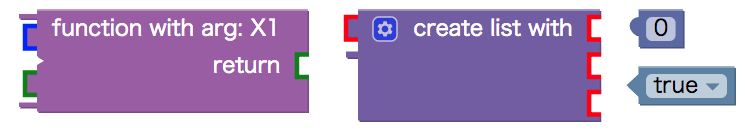
\includegraphics[scale=0.4]{img/blockEx.png}
 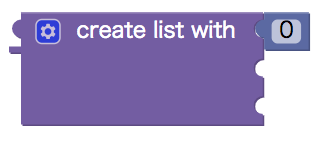
\includegraphics[scale=0.4]{img/intList.png} % TODO:余白合わせて!
 \caption{{\it Polymorphic Blocks}でのブロックの例.始めList型のパラメタの型は決定していないため,型変数を意味するハイライトが赤色で示されているが(中),Int型のブロックを接続させると,ハイライトが消えInt型の形に変更される(右).\label{fig:polyBlockList}}
 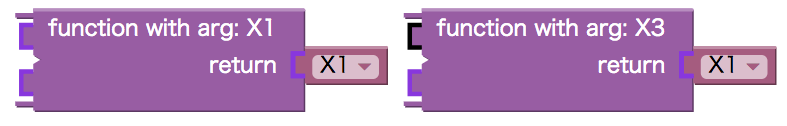
\includegraphics[scale=0.4]{img/unboundValue.png}
 \caption{{\it Polymorphic Blocks}で組み立てた2つのラムダ式ブロック.左のブロックはラムダ式として正当だが,右のブロックでは入れ子になったブロックが表す変数X1が未定義なってしまう.\label{fig:unboundValue}}
\end{figure}

他の関連研究としては,FunBlocks \cite{FunBlocks}がある.
これはCodeWorld \cite{CodeWorld} というHaskellプログラミングの学習環境をBlockly上に実現したものである.
\cite{Typed-Blockly}と同様に型や型変数を視覚的に描画する方法を取っているが,
let多相やブロックを外したときの型の単一化の解除を行うなど,型システムは\cite{Typed-Blockly}よりも拡張されている.
一方で,スコープという概念がないために図\ref{fig:unboundValue}と同じような不正なプログラムを表すブロックが組み立てられてしまう.
また,CodeWorld専用のプログラミング環境であるために,標準のOCamlエディタとして開発を行う本研究とは目的が異なる.

これらの点を踏まえて,本研究がOCaml Blocklyを開発する上で最終的に達成したい目標は以下の2点である.

\begin{itembox}[l]{本研究の掲げる最終的な目標}
  \begin {enumerate}
    \item {\bf 「穴のないブロックを組み立てられた」ならば「コンパイルエラーの起きないプログラム」である}ことを保証する.
    \item 関数型言語初学者向けの授業で使えるクオリティにする.
  \end {enumerate}
\end{itembox}

まず,1つ目の目標により,
コンパイルエラーの起きるプログラムを組み立てることを制限したユーザインタフェースを実装する.
この保証による利点は第\ref{chap:intro}節で述べた通りである.

続く2つ目の目標を達成するためにまず不可欠なことは,豊富な構文を揃えることである.
また,実際に授業で使用するためには初学者の視点から見た
「使いやすさ」「理解しやすさ」といった高いユーザビリティの達成は欠かすことができない.
そのためには,本来のBlockly にある直感的でわかりやすいユーザ体験を維持するだけでなく,
OCamlの言語仕様に特化したブロックのビジュアルを設計し,ブロックの表現を改造する必要がある.

一方で,「不正なプログラムを組み立てられない」という制約の元に,
授業で使う OCaml の全ての言語仕様をブロックで表現し,
なおかつ初学者が混乱しないユーザビリティを保つためには,多くの実装量が必要であることはもちろん,
実際に授業でユーザに体験してもらい,フィードバックをもらう必要がある.
そこで本論文では,最終的な目標を見据えた上で,そのproof of concept となる目標を実現する.
この目標は以下に示す通りで,それぞれの目標が最終的な目標のサブセットとなっていることに注意されたい.
\begin{itembox}[l]{本論文で実現される目標}
  \begin {enumerate}
    \item シンタックスエラー,型エラー,Unbound valueエラーが起きないことを保証する.
    \item 元のBlocklyの使いやすさを維持しつつ,OCamlに慣れるために必要な基礎的な構文を備える.
  \end {enumerate}
\end{itembox}

一概に「コンパイルエラー」と言ってもエラーの種類には様々なものがあるが,主なものは上で述べた3つである.
本論文では,
この3つのエラーを起こすプログラムを構成することができないようなユーザインタフェースを構築する.

構文のカバー範囲については,OCamlを使用言語とした「プログラミングの基礎」\cite{AsaiBook}の
前半部分で扱われるような,再帰関数,matchを用いたリストのパターンマッチなどを目標とし,
それらを「不正なプログラムを組み立てられない」という制約の元に実装する.

なお,\cite{Typed-Blockly}で行われた,
型をブロックのコネクタの形や色で表現するアイデアや一部の実装は継承する.
実装は,本来のBlocklyに合わせてJavaScriptで行う.
